\documentclass[tikz,border=2pt]{standalone}
\usepackage{amsmath}
\usepackage{tikz}

\begin{document}
% A \ B: the part of A that is not in B (shaded); B \ A is the other crescent.
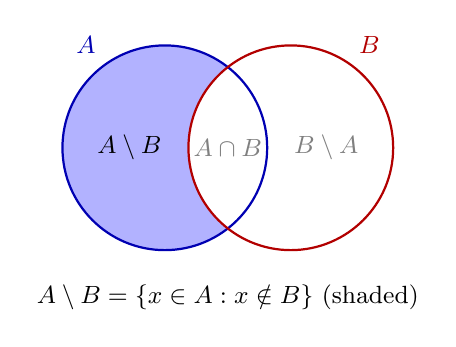
\begin{tikzpicture}[every node/.style={font=\small}]
	\begin{scope}
		\clip (0,0) circle (1.3);
		\fill[blue!30, even odd rule] (0,0) circle (1.3) (1.6,0) circle (1.3);
	\end{scope}
	\draw[thick, blue!70!black] (0,0) circle (1.3);
	\draw[thick, red!70!black] (1.6,0) circle (1.3);
	\node[blue!70!black] at (-1.0,1.3) {$A$};
	\node[red!70!black] at (2.6,1.3) {$B$};
	\node at (-0.45,0) {$A\setminus B$};
	\node[gray] at (0.8,0) {$A\cap B$};
	\node[gray] at (2.05,0) {$B\setminus A$};
	\node at (0.8,-1.9) {$A\setminus B=\{x\in A : x\notin B\}$ (shaded)};
\end{tikzpicture}
\end{document}
